\documentclass[notes=only]{beamer}
% \documentclass{beamer}
      
%% XeTeX preamble                                                                 
\usepackage{xltxtra}                      
\usepackage{hyperref}                                                           
\setmainfont[Mapping=tex-text]{DejaVu Serif}
\setsansfont[Mapping=tex-text]{DejaVu Sans}
\usepackage{polyglossia}                   
\setdefaultlanguage{russian}    
          
%% Commong preamble                                  
\usepackage{hyperref}                         
\usepackage{graphicx}

\usetheme{default} 
\setbeamertemplate{navigation symbols}{} 
\useoutertheme{infolines} 
\setbeamertemplate{footline}{
  \scriptsize{\hfill\insertframenumber/\inserttotalframenumber\hspace*{.2cm}}
} 

\title{Оконное преобразование Уолша}
\author[Григорий Калабин]{Калабин Григорий Александрович, 523 группа
  \\{\footnotesize Научный руководитель: к.\,ф.-м.\,н., доц. С.М.~Машарский}
  \\{\footnotesize Рецензент: д.\,ф.-м.\,н., проф. В.Н.~Малозёмов}
}
\institute[СПбГУ]{Санкт-Петербургский Государственный Университет\\Математико-Механический факультет\\ Кафедра Исследования Операций}
\date{Весна, 2013}
\titlegraphic{
\includegraphics[width=1.8cm]{spbu-logo}}

\begin{document}
    \frame{
    \titlepage
    \note{Здравствуйте, меня зовут Григорий Калабин, мой научный руководитель ---
    Сергей Михайлович Машарский, а рецензент --- Василий Николаевич Малозёмов.
    Тема моей дипломной работы --- Оконное преобразование Уолша.
    Я применяю данный подход для обработки цифровых дискретных аудио сигналов,
    поэтому для начала я расскажу про особенности их обработки
    }
    }
    
%%%%%%%%%%%%%%%%%%%%%%%%%%%%%%%%%%%%%%%%%%%%%%%%%%%%%%%%%%%%%%%%%%%%%%%%%%%%%%%%
  
\begin{frame}\frametitle{Особенности обработки сигналов}
\begin{itemize}
    \item Сигнал может быть достаточно длинным
    \item 44.1~kHz = 44 100 значений в секунду \\
        2 минуты такого аудио --- 5~292~000 отсчётов
    \item<2-> Изменения аудио во время прослушивания \\
        Пример: эквализация
    \item<3-> Обработка сигнала в реальном времени \\
        Пример: передача голоса
\end{itemize}

\note<1>{
  Первое, что нужно учитывать при обработке аудио, то, что
  объёмы данных могут быть достаточно большими, поэтому обрабатывать
  сигналы необходимо с помощью быстрых алгоритмов
}
\note<2>{
  Зачастую возникает необходимость изменять сигнал во время прослушивания.
  Подобная ситуация возникает при работе с эквалайзером, например, когда
  мы хотим устранить некоторые шумы.
}
\note<3>{
  Ещё одна особенность, часто встречающаяся в наши дни --- потоковая обработка
  аудиосигналов. Например, когда мы разговариваем по телефону, наш голос
  оцифровывается, проходит обработку (такую, как шумоподавление и эхоподавление)
  и передаётся собеседнику.
  Априори неизвестно сколько продлится разговор, и обрабатывать сигнал нужно
  в реальном времени.
}
\note{
  Теперь рассмотрим определения объектов, используемых в работе
}
\end{frame}
    
%%%%%%%%%%%%%%%%%%%%%%%%%%%%%%%%%%%%%%%%%%%%%%%%%%%%%%%%%%%%%%%%%%%%%%%%%%%%%%%%
  
\begin{frame}\frametitle{Предварительные сведения}
  \emph{Сигналом} длины $N \in \mathbb{N}$ будем называть функцию x:
  \begin{equation}
    x:\: \mathbb{Z} \rightarrow \mathbb{C}, \quad \mathrm{supp} (x) = 0:N-1 
  \end{equation}

  Множество сигналов обозначим как $\mathbb{C}_N$.

  \emph{Потоком данных} будем называть бесконечный в обе стороны сигнал.
  
  \note{
    Сигналом длины N будем называть целочисленную функцию комплексного аргумента
    с носителем от нуля до $N$.
    \\
    Пространство сигналов обозначим как $\mathbb{C}_N$.
    Поток данных --- бесконечный в обе стороны сигнал
  }
\end{frame}
    
%%%%%%%%%%%%%%%%%%%%%%%%%%%%%%%%%%%%%%%%%%%%%%%%%%%%%%%%%%%%%%%%%%%%%%%%%%%%%%%%
  
\begin{frame}\frametitle{Предварительные сведения}
Рассмотрим 
\[
N = 2^s, \; \Delta_\nu = 2^{\nu - 1}.
\]

Пусть 
\[
k,j \in 0 : \Delta_{\nu+1}-1, \;
\]
\[
k=(k_{\nu-1},k_{\nu-2},\ldots,k_0)_2 \, , \: 
j=(j_{\nu-1},j_{\nu-2},\ldots,j_0)_2. 
\]

Положим 
\[
\{k,j\}_\nu = \sum_{\alpha=0}^{\nu-1} k_\alpha j_\alpha \; , \quad k,j \in 0: \Delta_{\nu+1} - 1.
\]
Функции 
\begin{equation}
v_k(j) = (-1)^{{\{k,j\}}_s} \;, \qquad k,j \in 0:N-1
\end{equation}
называются \emph{дискретными функциями Уолша}.


\note{
  Мы будем рассматривать сигналы, длина которых представляется степенью двойки.
  Дискретными функциями Уолша называются функции, задаваемые формулой два.
}
\end{frame}
    
%%%%%%%%%%%%%%%%%%%%%%%%%%%%%%%%%%%%%%%%%%%%%%%%%%%%%%%%%%%%%%%%%%%%%%%%%%%%%%%%
  
\begin{frame}\frametitle{Предварительные сведения}
Дискретные функции Уолша образуют базис в $\mathbb{C}_N$. 
Этот базис называется \emph{базисом Уолша-Адамара}.

Пусть $j \in 0:2^\nu - 1$ и $j=(j_{\nu-1}, j_{\nu-2}, \ldots, j_0)_2$.
Введём обозначение  
\[
  \mathrm{rev}_\nu(j) = (j_0, j_1, \ldots, j_{\nu-1})_2.
\]

Частота функции $v_k$ равна $\mathrm{rev}_s(k)$. 

Обозначим
$\hat{v}_k = v_{\mathrm{rev}_s(k)}$. 

Функции $\hat{v}_k$ тоже образуют
ортогональный базис
в пространстве $\mathbb{C}_N$ который называется \emph{базисом Уолша-Пэли}.

\begin{equation}
  x = \frac{1}{N} \sum_{k=0}^{N-1} X(k) v_k = 
  \frac{1}{N} \sum_{k=0}^{N-1} X(\mathrm{rev}_s(k)) \hat{v}_k.
\end{equation}

\note{
  Известно, что функции Уолша образуют базис в $\mathbb{C}_N$, 
  этот базис называется базисом Уолша-Адамара.
  Переупорядочим функции $v_k$ по частоте, получим базис Уолша-Пэли, его и будем
  использовать.
}
\end{frame}
    
%%%%%%%%%%%%%%%%%%%%%%%%%%%%%%%%%%%%%%%%%%%%%%%%%%%%%%%%%%%%%%%%%%%%%%%%%%%%%%%%
  
\begin{frame}\frametitle{Дискретные функции Уолша при $N=2^3$}
\begin{figure}
    \centering
    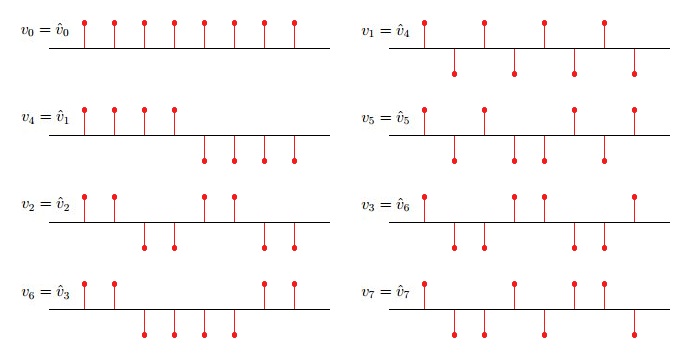
\includegraphics[width=\textwidth]{../images/walsh.png}
\end{figure}

\note{
  На рисунке представлены функции Уолша для $N=8$
}
\end{frame}
    
%%%%%%%%%%%%%%%%%%%%%%%%%%%%%%%%%%%%%%%%%%%%%%%%%%%%%%%%%%%%%%%%%%%%%%%%%%%%%%%%
  
\begin{frame}\frametitle{Вычисление спектра Уолша}
Будем использовать разложение сигнала по базису Уолша-Пэли, так как
этот базис упорядочен по частоте.

Поэтому необходимо уметь вычислять коэффициенты разложения сигнала по
базису Уолша-Пэли.

Будем использовать быстрое преобразование Уолша, связанное с прореживанием
по времени. Эта схема использует сложения в количестве 
$N\log_2 N$ операций
и допускает обращение с той же скоростью.

\note{
  Для вычисления компонент разложения по базису Уолша-Пели будем использовать
  быстрое преобразование Уолша со скоростью $N \log_2 N$
}
\end{frame}
    
    
%%%%%%%%%%%%%%%%%%%%%%%%%%%%%%%%%%%%%%%%%%%%%%%%%%%%%%%%%%%%%%%%%%%%%%%%%%%%%%%%
    
\begin{frame}\frametitle{Оконная функция}
\emph{Оконной функцией}, или \emph{окном}, называется весовая функция, которая равна нулю вне заданного
интервала. Например, \emph{прямоугольное окно}:
$$
w_{rect}(k) = 
\left\{ \begin{array}{ll}
  1, & \textrm{если} \; L \leq k \leq R  \\
  0, & \textrm{иначе}
\end{array} \right.
$$
где $[L;R]$ --- заданный интервал.

\note{
  Оконной функцией будем называть весовую функцию, равную нулю вне заданного 
  интервала.
}
\end{frame}
    
%%%%%%%%%%%%%%%%%%%%%%%%%%%%%%%%%%%%%%%%%%%%%%%%%%%%%%%%%%%%%%%%%%%%%%%%%%%%%%%%

\begin{frame}\frametitle{Идея оконного преобразования}
Имеется исходный поток данных, который необходимо обработать.

\begin{enumerate}
  \item Зафиксируем $N \in \mathbb{N}$.
  \item Определим сигнал $x$, как очередные $N$ отсчётов исходного потока данных. 
  \item Произведём обработку $x$ и получим $x' \in \mathbb{C}_N$.
  \item Запишем $x'$ в некоторый буфер.
  \item Будем повторять шаги 2--4 пока не обработаем весь поток данных.
    Буфер будет содержать результат обработки исходного потока.
\end{enumerate}

\note{
  Длиной окна будем называть натуральное число $N$.\\
  Возьмём очередные $N$ отсчётов исходного потока данных, обработаем их и запишем
  в некий буфер.\\
  Будем повторять процедуру, пока не закончим обработку, в итоге буфер будет
  содержать результат обработки.\\
  Формальные определения прямого и обратного преобразования Уолша даны на следующих двух слайдах
}
\end{frame}
    
%%%%%%%%%%%%%%%%%%%%%%%%%%%%%%%%%%%%%%%%%%%%%%%%%%%%%%%%%%%%%%%%%%%%%%%%%%%%%%%%
  
\begin{frame}\frametitle{Определение оконного преобразования Уолша}
Пусть у нас есть
некоторый поток данных $x$ и прямоугольная оконная функция $w$ с носителем
$0:N-1$.

Оконным преобразованием Уолша потока данных $x$ называется матрица $X$, задаваемая 
следующим равенством:

\begin{equation}
\mathbf{STWT}\{x\}(d,k)\equiv X(d,k) 
= \frac{1}{N} \sum_{j=0}^{N-1} x[j+d]w[j]\hat{v}_k(j),
\end{equation}

где $k \in 0:N-1, \; d \in (-\infty; +\infty)$. 
Индекс $d$ матрицы соответствует точке во времени, а индекс $k$ --- частоте.
Таким образом, данная матрица позволяет по времени и частоте узнать 
магнитуду исходного сигнала.

\note{
  прямое... (раз-два-три)
}
\end{frame}
    
%%%%%%%%%%%%%%%%%%%%%%%%%%%%%%%%%%%%%%%%%%%%%%%%%%%%%%%%%%%%%%%%%%%%%%%%%%%%%%%%
  
\begin{frame}\frametitle{Обратное оконное преобразование Уолша}
Для каждого оконного спектра $X(d, k)$ вычислим обратное преобразование
Уолша и получим часть исходного потока данных:
\[
x(d,j) = \sum_{k=0}^{N-1} X(d,k) \hat{v}_k(j),
\quad j \in 0:N-1, \; d \in (-\infty; +\infty).
\]

Поскольку в данной работе рассматривается оконное преобразование
с прямоугольным окном, то
можно перейти от матрицы $x(d,j)$ к исходному потоку данных $x(t)$ следующим образом:
\begin{equation}
 x(t) = \frac{1}{N} \sum_{j=0}^{N-1} x(t-j,j), \quad t \in (-\infty; +\infty).
\end{equation}

\note{
  и обратное... (раз-два-три)
}
\end{frame}

%%%%%%%%%%%%%%%%%%%%%%%%%%%%%%%%%%%%%%%%%%%%%%%%%%%%%%%%%%%%%%%%%%%%%%%%%%%%%%%%
  
\begin{frame}\frametitle{Результаты}
В рамках данной работы было реализовано оконное преобразование Уолша на языке java
и были проведены различные эксперименты. 

\begin{table}
  \centering
    \resizebox{\textwidth}{!} {
    \begin{tabular}{ | c | c | r | r | p{4.5cm} |}
    \hline
    Название & Инструмент & Длит. & Размер, bytes (samples) & Примечание \\ \hline
    vivaldi.wav & Скрипка & 15~сек & 2 921 548 (1 460 752) & Антонио Вивальди, <<Весна>>, часть 1 Аллегро \\ \hline
    chopin.wav & Фортепиано & 13~сек & 1 178 548 (589 203) & Фридерик Шопен, <<ноктюрн №2>> \\ \hline
    metallica.wav & Гитара & 24~сек & 2 190 902 (1 095 429) & Группа <<Metallica>>, <<Nothing else matters>> \\ \hline
    voice.wav & Речь & 3~сек & 702 644 (351 300) & Женская речь \\ \hline
    \end{tabular}}
\end{table}

Было установлено, что при помощь оконного преобразования Уолша возможна
достаточно эффективная обработка сигналов.

\note{
  В рамках данной работы были написаны два приложения для демонстрации того, что
  с помощью оконного преобразования Уолша возможна эффективная обработка сигналов.
  \\
  Были проведены различные эксперименты на различных аудиозаписях, информация
  о которых представлена в таблице.
}
\end{frame}
    
%%%%%%%%%%%%%%%%%%%%%%%%%%%%%%%%%%%%%%%%%%%%%%%%%%%%%%%%%%%%%%%%%%%%%%%%%%%%%%%%
  
\begin{frame}\frametitle{Фильтрация частот}
Был проведён эксперимент в котором из спектра вырезались верхние частоты, то есть
к исходному сигналу применялся простейший низкочастотный фильтр.

При проведении эксперимента использовалось прямоугольное окно без наложений с длиной
равной 4096 отсчётам.

В результате было получено,
что при вырезании $15/16$ верхних частот результат фильтрации вполне узнаваем.
Можно сделать вывод, что верхние частоты при разложении сигнала по
базису Уолша воспринимаются человеком значительно меньше, чем низкие.

\note{
  Первым приложением написаным в рамках данной работы является эквалайзер.
  С его помощью можно изменять мощность восьми диапазонов частот.
  
  Выяснилось, что при обнулении $15/16$ верхних частот результат вполне различим.
  Этот факт говорит о том, что возможно эффективно сжимать аудио с помощью
  оконного преобразования Уолша, например, для передачи информации по узким
  каналам связи.
}
\end{frame}
    
%%%%%%%%%%%%%%%%%%%%%%%%%%%%%%%%%%%%%%%%%%%%%%%%%%%%%%%%%%%%%%%%%%%%%%%%%%%%%%%%
  
\begin{frame}\frametitle{Сжатие звука}
Для сжатия данных использовался алгоритм DEFLATE.

Компрессия применялась не к каждому отдельному окну, а ко всему
сигналу целиком.

\begin{table}
  \centering
    \resizebox{\textwidth}{!} {
    \begin{tabular}{ | p{2.6cm} | r | r | r | r |}
    \hline
    Название файла & Без фильтрации & 1/2 спектра & 1/4 спектра & 1/8 спектра \\ \hline
    vivaldi.wav     & 1.25  & 2.32  & 4.36  & 8.21 \\ \hline
    metallica.wav   & 1.22  & 2.28  & 4.32  & 8.15 \\ \hline
    chopin.wav      & 1.21  & 2.27  & 4.31  & 8.11 \\ \hline
    voice.wav       & 1.21  & 2.26  & 4.27  & 8.10 \\ \hline
    \end{tabular}}
\end{table}

\note{
  Второе приложение, написанное в рамках данной работы позволяет сжимать аудио
  на основе оконного преобразования Уолша. В таблице представлены коэффициенты сжатия
  при указанной ненулевой части спектра.
}
\end{frame}
    
%%%%%%%%%%%%%%%%%%%%%%%%%%%%%%%%%%%%%%%%%%%%%%%%%%%%%%%%%%%%%%%%%%%%%%%%%%%%%%%%
  
\begin{frame}
 \frametitle{Список литературы}
 \begin{thebibliography}{9}    
  \setbeamertemplate{bibliography item}[book]
  \bibitem{dha}
    В.Н.~Малоземов, С.М.~Машарский,
    {\em Основы дискретного гармонического анализа}.
    \newblock СПб.:~Лань, 2012 --- 304~с.
  \setbeamertemplate{bibliography item}[article]
  \bibitem{allen}
    Jont~B.Allen,
    {\em Short Term Spectral Analysis, Synthesis, and Modification by Discrete Fourier Transform}.
    \newblock IEEE Transactions on acoustics, speech, and signal processing, \textbf{ASSP--25}~(1977), no.~3, p.~235--238.
  \setbeamertemplate{bibliography item}{
\includegraphics[width=1.5em]{../images/beamericononline.eps}}
  \bibitem{wav-spec}
    Prof. Peter Kabal,
    {\em The WAVE file specifications}, 2011.
    \newblock \url{http://www-mmsp.ece.mcgill.ca/Documents/AudioFormats/WAVE/WAVE.html}
  \setbeamertemplate{bibliography item}{
\includegraphics[width=1.5em]{../images/beamericononline.eps}}
  \bibitem{deflate-spec}
    Phil Katz,
    {\em DEFLATE Compressed Data Format Specification}, 1996.
    \newblock \url{http://tools.ietf.org/html/rfc1951}
  \end{thebibliography}
\end{frame}
    
%%%%%%%%%%%%%%%%%%%%%%%%%%%%%%%%%%%%%%%%%%%%%%%%%%%%%%%%%%%%%%%%%%%%%%%%%%%%%%%%
  
\begin{frame}[c]
\begin{center}
{\Large \textcolor{blue}{Спасибо!}}
\end{center}
\end{frame}
    
%%%%%%%%%%%%%%%%%%%%%%%%%%%%%%%%%%%%%%%%%%%%%%%%%%%%%%%%%%%%%%%%%%%%%%%%%%%%%%%%

    
\end{document}